\chapter{Relazioni tra grandezze}

In fisica due grandezze sono quasi sempre \textbf{legate} l'una all'altra: se se ne cambia una, cambia anche l'altra. L'allungamento di una molla dipende dalla forza applicata; il volume di un liquido versato in un bicchiere dipende dall'altezza che raggiunge; il tempo di un viaggio dipende dalla velocità. Riconoscere \emph{che tipo} di legame c'è fra due grandezze -- e saperlo leggere da una tabella o da un grafico -- è uno degli obiettivi di ogni esperimento.

In questo capitolo studiamo i tre legami più semplici e più frequenti: la \textbf{proporzionalità diretta}, la \textbf{proporzionalità inversa} e la \textbf{proporzionalità quadratica}. Per ciascuno vedremo la formula, il grafico e alcuni esempi, sia geometrici sia fisici, con numeri semplici.

\section{La proporzionalità diretta}

\begin{definizione}
Due grandezze $x$ e $y$ sono \textbf{direttamente proporzionali} quando il loro \textbf{rapporto è costante}:
\[ \colorboxed{ocre}{ \frac{y}{x} = k \qquad\text{ovvero}\qquad y = k\,x. } \]
La costante $k$ si chiama \textbf{costante di proporzionalità}.
\end{definizione}

La proprietà che si ricorda più facilmente è questa: \textbf{se $x$ raddoppia, anche $y$ raddoppia}; se $x$ diventa tre volte più grande, anche $y$ diventa tre volte più grande; se $x$ si dimezza, anche $y$ si dimezza. In particolare, quando $x = 0$ anche $y = 0$.

\subsection{Il grafico}
Riportando su un grafico cartesiano $x$ in ascissa e $y$ in ordinata, i punti di due grandezze direttamente proporzionali si dispongono lungo una \textbf{retta che passa per l'origine} (figura~\ref{fig:rel-diretta}). La pendenza di questa retta è proprio la costante $k$.

\begin{figure}[!htbp]
    \centering
    \begin{tikzpicture}
    \begin{axis}[
        width=0.6\linewidth, height=5cm,
        xlabel={$x$}, ylabel={$y$},
        xmin=0, xmax=5.5, ymin=0, ymax=11,
        xtick=\empty, ytick=\empty,
        axis lines=left,
    ]
    \addplot[ocre, very thick, domain=0:5] {2*x};
    \addplot[only marks, mark=*, mark size=1.4pt, black]
        coordinates {(1,2)(2,4)(3,6)(4,8)(5,10)};
    \node[ocre, anchor=west] at (axis cs:3.1,5.4) {$y = k\,x$};
    \end{axis}
    \end{tikzpicture}
    \caption{Grafico di due grandezze direttamente proporzionali: una retta passante per l'origine, di pendenza $k$.}
    \label{fig:rel-diretta}
\end{figure}

\subsection{Esempi geometrici}
\begin{itemize}
    \item \textbf{Circonferenza e raggio.} La lunghezza di una circonferenza è $C = 2\pi\,r$. Il rapporto $C/r = 2\pi \approx 6{,}28$ è lo stesso per qualunque cerchio: $C$ ed $r$ sono direttamente proporzionali, con costante $k = 2\pi$. Raddoppiando il raggio, raddoppia la circonferenza.
    \item \textbf{Perimetro di un quadrato e lato.} $P = 4\,l$: la costante è $k = 4$.
\end{itemize}

\subsection{Il volume di un liquido in un contenitore cilindrico}
Versiamo dell'acqua in un cilindro graduato la cui base ha area $A$ (figura~\ref{fig:cilindro-h}). Il volume di liquido contenuto è
\[ V = A\,h, \]
dove $h$ è l'altezza raggiunta dal liquido. Se il contenitore è sempre lo stesso, $A$ è fissa e funziona da costante di proporzionalità: \textbf{il volume è direttamente proporzionale all'altezza}. Ecco perché sul cilindro graduato la scala delle tacche è \emph{uniforme}: a intervalli di altezza uguali corrispondono volumi uguali.

\begin{figure}[!htbp]
    \centering
    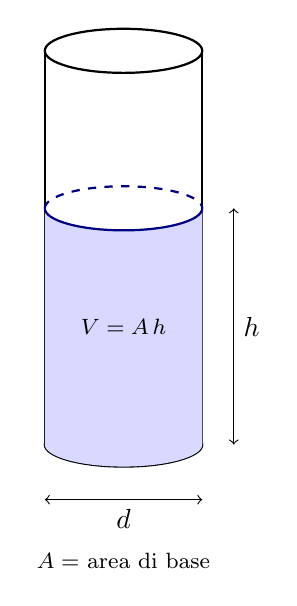
\begin{tikzpicture}[scale=1]
        % fondo
        \draw[thick,dashed] (-1,0) arc (180:0:1 and 0.28);
        \draw[thick] (-1,0) arc (180:360:1 and 0.28);
        % pareti
        \draw[thick] (-1,0) -- (-1,5);
        \draw[thick] (1,0) -- (1,5);
        % bordo superiore
        \draw[thick] (0,5) ellipse (1 and 0.28);
        % liquido (livello a 3)
        \fill[blue!15] (-1,0) -- (-1,3) arc (180:360:1 and 0.28) -- (1,0) arc (360:180:1 and 0.28);
        \draw[blue!50!black,thick] (-1,3) arc (180:360:1 and 0.28);
        \draw[blue!50!black,thick,dashed] (-1,3) arc (180:0:1 and 0.28);
        % quote
        \draw[<->] (1.4,0) -- (1.4,3) node[midway,right]{$h$};
        \draw[<->] (-1,-0.7) -- (1,-0.7) node[midway,below]{$d$};
        \node at (0,1.5) {\footnotesize $V = A\,h$};
        \node[below] at (0,-1.25) {\footnotesize $A = $ area di base};
    \end{tikzpicture}
    \caption{In un contenitore cilindrico il volume di liquido è $V = A\,h$: a base fissa, $V$ è direttamente proporzionale all'altezza $h$.}
    \label{fig:cilindro-h}
\end{figure}

\begin{testexample}[\thetcbcounter \, Lettura di un cilindro graduato]
Un cilindro graduato ha base di area $A = \SI{20}{\centi\metre\squared}$. Che volume di liquido contiene quando il livello è a \SI{6}{\centi\metre}? E a \SI{9}{\centi\metre}?
\[ V_1 = A\,h_1 = 20 \cdot 6 = \SI{120}{\centi\metre\cubed}, \qquad
   V_2 = A\,h_2 = 20 \cdot 9 = \SI{180}{\centi\metre\cubed}. \]
Passando da \SI{6}{\centi\metre} a \SI{9}{\centi\metre} l'altezza è aumentata di una volta e mezza, e il volume è passato da \SI{120}{} a \SI{180}{\centi\metre\cubed}: anch'esso di una volta e mezza.
\end{testexample}

\subsection{Esempi fisici}
\begin{itemize}
    \item \textbf{Massa e volume.} Per un dato materiale, la massa è direttamente proporzionale al volume: $m = \rho\,V$, dove la costante $\rho$ è la \emph{densità} (capitolo~1). Un blocco di ferro di \SI{20}{\centi\metre\cubed} ha massa doppia di uno di \SI{10}{\centi\metre\cubed} dello stesso materiale.
    \item \textbf{Forza e allungamento di una molla.} Entro certi limiti, l'allungamento di una molla è direttamente proporzionale alla forza applicata: $F = k\,\Delta x$ (legge di Hooke), con $k$ costante elastica. La studierai fra i capitoli sulle forze.
    \item \textbf{Spazio e tempo nel moto uniforme.} Un corpo che si muove a velocità costante percorre spazi direttamente proporzionali ai tempi: $s = v\,t$, con costante $v$.
\end{itemize}

\begin{esercizio}
Il perimetro di un quadrato misura \SI{14}{\centi\metre}. Quanto misura il lato? E se il perimetro fosse \SI{30}{\centi\metre}?\\
\risp{$l = \SI{3,5}{\centi\metre}$; \; $l = \SI{7,5}{\centi\metre}$}
\end{esercizio}

\begin{esercizio}
Una molla ha costante elastica $k = \SI{25}{\newton\per\metre}$. Che forza serve per allungarla di \SI{8,0}{\centi\metre}? Di quanto si allunga con una forza di \SI{5,0}{\newton}?\\
\risp{$F = \SI{2,0}{\newton}$; \; $\Delta x = \SI{20}{\centi\metre}$}
\end{esercizio}

\begin{esercizio}
L'alluminio ha densità \SI{2,70}{\gram\per\centi\metre\cubed}. Qual è la massa di \SI{50}{\centi\metre\cubed} di alluminio? Che volume occupano \SI{216}{\gram} di alluminio?\\
\risp{$m = \SI{135}{\gram}$; \; $V = \SI{80}{\centi\metre\cubed}$}
\end{esercizio}

\begin{esercizio}
In un cilindro graduato di base \SI{15}{\centi\metre\squared} il liquido arriva a \SI{8,0}{\centi\metre}. Che volume contiene? A quale altezza arriverebbe un volume di \SI{180}{\centi\metre\cubed}?\\
\risp{$V = \SI{120}{\centi\metre\cubed}$; \; $h = \SI{12}{\centi\metre}$}
\end{esercizio}

\section{La proporzionalità inversa}

\begin{definizione}
Due grandezze $x$ e $y$ sono \textbf{inversamente proporzionali} quando il loro \textbf{prodotto è costante}:
\[ \colorboxed{ocre}{ x\,y = k \qquad\text{ovvero}\qquad y = \frac{k}{x}. } \]
\end{definizione}

Qui la regola da ricordare è opposta a prima: \textbf{se $x$ raddoppia, $y$ si dimezza}; se $x$ diventa tre volte più grande, $y$ diventa tre volte più piccolo. Le due grandezze ``si compensano'' in modo che il loro prodotto resti sempre lo stesso.

\subsection{Il grafico}
Il grafico di due grandezze inversamente proporzionali è una \textbf{curva discendente} chiamata \emph{iperbole} (figura~\ref{fig:rel-inversa}): parte da valori molto grandi quando $x$ è piccolo, poi scende avvicinandosi all'asse orizzontale senza mai toccarlo. Attenzione: \emph{molte} curve scendono in quel modo, quindi il grafico da solo non basta a dire che la proporzionalità è inversa. La prova certa è che il \textbf{prodotto $x\,y$ risulti costante} (lo vedremo nel paragrafo~\ref{sec:riconoscere}).

\begin{figure}[!htbp]
    \centering
    \begin{tikzpicture}
    \begin{axis}[
        width=0.6\linewidth, height=5cm,
        xlabel={$x$}, ylabel={$y$},
        xmin=0, xmax=6, ymin=0, ymax=13,
        xtick=\empty, ytick=\empty,
        axis lines=left,
    ]
    \addplot[ocre, very thick, samples=80, domain=0.9:6] {12/x};
    \addplot[only marks, mark=*, mark size=1.4pt, black]
        coordinates {(1,12)(2,6)(3,4)(4,3)(6,2)};
    \node[ocre, anchor=west] at (axis cs:2.6,5.5) {$y = \dfrac{k}{x}$};
    \end{axis}
    \end{tikzpicture}
    \caption{Grafico di due grandezze inversamente proporzionali: un'iperbole. Il prodotto $x\,y$ è lo stesso per tutti i punti.}
    \label{fig:rel-inversa}
\end{figure}

C'è però un trucco utile: se al posto di $x$ mettiamo in ascissa il suo \textbf{reciproco} $1/x$, allora $y = k\cdot(1/x)$ e il grafico di $y$ in funzione di $1/x$ diventa una \textbf{retta passante per l'origine}. Trasformare una curva in una retta scegliendo la variabile giusta si chiama \emph{linearizzazione}, ed è una tecnica che si usa spesso in laboratorio.

\subsection{Esempi geometrici e fisici}
\begin{itemize}
    \item \textbf{Rettangoli di area fissa.} Se vogliamo che un rettangolo abbia sempre area $A = \SI{24}{\centi\metre\squared}$, base e altezza sono inversamente proporzionali: $b\,h = 24$. Con base \SI{4}{\centi\metre} l'altezza è \SI{6}{\centi\metre}; con base \SI{8}{\centi\metre} (doppia) l'altezza è \SI{3}{\centi\metre} (metà).
    \item \textbf{Stessa distanza a velocità diverse.} Per percorrere \SI{120}{\kilo\metre}, a \SI{60}{\kilo\metre\per\hour} servono \SI{2}{\hour}, a \SI{120}{\kilo\metre\per\hour} ne serve \SI{1}{}: velocità e tempo sono inversamente proporzionali, $v\,t = \SI{120}{\kilo\metre}$.
    \item \textbf{Pressione e volume di un gas.} Comprimendo un gas a temperatura costante, se il volume si dimezza la pressione raddoppia: $p\,V$ resta costante (legge di Boyle).
\end{itemize}

\begin{remark}
Nel capitolo precedente (``Grafici di misure'') avevamo osservato che la capacità di un condensatore \emph{diminuisce} all'aumentare della distanza fra le armature, e avevamo detto che era un \emph{indizio} di proporzionalità inversa. Ora sappiamo come verificarlo davvero: bisogna controllare se il prodotto (capacità)$\times$(distanza) si mantiene costante.
\end{remark}

\begin{testexample}[\thetcbcounter \, Operai e giorni di lavoro]
Un muretto viene costruito da \SI{12}{} operai in \SI{15}{} giorni. Supponendo che tutti lavorino allo stesso ritmo, quanti giorni impiegherebbero \SI{20}{} operai?

Il ``lavoro totale'' si può misurare in \emph{giornate-uomo}: $12 \cdot 15 = 180$. Questo numero è la costante. Con \SI{20}{} operai:
\[ t = \frac{180}{20} = \SI{9}{giorni}. \]
Più operai, meno giorni: numero di operai e giorni sono inversamente proporzionali.
\end{testexample}

\begin{esercizio}
Un rettangolo deve avere area \SI{36}{\metre\squared}. Qual è l'altezza se la base è \SI{9}{\metre}? E la base se l'altezza è \SI{3}{\metre}?\\
\risp{$h = \SI{4}{\metre}$; \; $b = \SI{12}{\metre}$}
\end{esercizio}

\begin{esercizio}
Una pompa comprime \SI{3,0}{\litre} di aria da \SI{1,0}{\bar} fino a un volume di \SI{1,2}{\litre}, a temperatura costante. Qual è la nuova pressione?\\
\risp{$p = \SI{2,5}{\bar}$}
\end{esercizio}

\begin{esercizio}
Per un viaggio di \SI{300}{\kilo\metre}, un automobilista impiega \SI{5,0}{\hour}. Quanto tempo impiegherebbe raddoppiando la velocità media? E se la velocità media fosse un terzo?\\
\risp{$\SI{2,5}{\hour}$; \; $\SI{15}{\hour}$}
\end{esercizio}

\section{La proporzionalità quadratica}

\begin{definizione}
Una grandezza $y$ è \textbf{proporzionale al quadrato} di un'altra grandezza $x$ quando
\[ \colorboxed{ocre}{ \frac{y}{x^2} = k \qquad\text{ovvero}\qquad y = k\,x^2. } \]
\end{definizione}

Stavolta la regola è: \textbf{se $x$ raddoppia, $y$ diventa quattro volte più grande} (perché $2^2 = 4$); se $x$ triplica, $y$ diventa nove volte più grande ($3^2 = 9$). La grandezza $y$ ``cresce molto più in fretta'' di $x$.

\subsection{Il grafico}
Il grafico di $y = k\,x^2$ è un ramo di \textbf{parabola} (figura~\ref{fig:rel-quadratica}): parte piano vicino all'origine e poi sale sempre più ripido. Come per la proporzionalità inversa, la prova certa non è la forma del grafico ma il fatto che il rapporto $y/x^2$ sia costante. E anche qui c'è una linearizzazione: se in ascissa mettiamo $x^2$ invece di $x$, il grafico diventa una retta per l'origine.

\begin{figure}[!htbp]
    \centering
    \begin{tikzpicture}
    \begin{axis}[
        width=0.6\linewidth, height=5cm,
        xlabel={$x$}, ylabel={$y$},
        xmin=0, xmax=5.5, ymin=0, ymax=27,
        xtick=\empty, ytick=\empty,
        axis lines=left,
    ]
    \addplot[ocre, very thick, samples=60, domain=0:5] {x^2};
    \addplot[only marks, mark=*, mark size=1.4pt, black]
        coordinates {(1,1)(2,4)(3,9)(4,16)(5,25)};
    \node[ocre, anchor=east] at (axis cs:4.2,22) {$y = k\,x^2$};
    \end{axis}
    \end{tikzpicture}
    \caption{Grafico di una proporzionalità quadratica: un ramo di parabola. Il rapporto $y/x^2$ è costante.}
    \label{fig:rel-quadratica}
\end{figure}

\subsection{Esempi}
\begin{itemize}
    \item \textbf{Area di un quadrato e lato.} $A = l^2$: raddoppiando il lato, l'area quadruplica. Una piastrella di \SI{40}{\centi\metre} di lato copre quattro volte la superficie di una da \SI{20}{\centi\metre}.
    \item \textbf{Area di un cerchio e raggio.} $A = \pi\,r^2$: la costante è $k = \pi$. Un cerchio di raggio triplo ha area nove volte maggiore.
    \item \textbf{Caduta libera.} Un corpo lasciato cadere (senza attrito dell'aria) percorre uno spazio proporzionale al \emph{quadrato} del tempo: $s = \tfrac{1}{2}\,g\,t^2$. Nel primo secondo cade circa \SI{4,9}{\metre}, in due secondi circa \SI{19,6}{\metre} (quattro volte tanto). Lo studierai nel capitolo sul moto.
\end{itemize}

\begin{testexample}[\thetcbcounter \, Il prezzo della pizza]
Una pizzeria vende una pizza di diametro \SI{30}{\centi\metre} a \SI{8,00}{euro}. Quanto dovrebbe costare, allo stesso prezzo al centimetro quadrato, una pizza di diametro \SI{45}{\centi\metre}?

Ciò che si paga è la \emph{superficie}, e la superficie è proporzionale al quadrato del diametro. Il diametro passa da \SI{30}{} a \SI{45}{\centi\metre}, cioè diventa $45/30 = 1{,}5$ volte:
\[ \text{area} \times (1{,}5)^2 = \text{area} \times 2{,}25. \]
Il prezzo equo sarebbe $8{,}00 \cdot 2{,}25 = \SI{18,00}{euro}$. La pizza ``grande'' contiene molta più pizza di quanto suggerisca il solo diametro!
\end{testexample}

\begin{esercizio}
Un quadrato ha lato \SI{6}{\centi\metre}. Come cambia la sua area se il lato triplica?\\
\risp{diventa $9$ volte più grande ($\SI{36}{} \to \SI{324}{\centi\metre\squared}$)}
\end{esercizio}

\begin{esercizio}
Il raggio di un cerchio passa da \SI{5}{\centi\metre} a \SI{20}{\centi\metre}. Di quante volte aumenta l'area?\\
\risp{$16$ volte}
\end{esercizio}

\begin{esercizio}
Nella tabella, $y$ è proporzionale al quadrato di $x$: $x = 1,2,3,4$ dà $y = 5,20,45,80$. Qual è la costante $k$? Quanto vale $y$ per $x = 10$?\\
\risp{$k = 5$; \; $y = \SI{500}{}$}
\end{esercizio}

\section{Quando l'inverso incontra il quadrato}

Diretta, inversa e quadratica si possono combinare. Il caso più comune è quello in cui una grandezza è \textbf{inversamente proporzionale al quadrato} di un'altra:
\[ y = \frac{k}{x^2}, \qquad\text{ossia}\qquad y\,x^2 = k. \]
Qui, \textbf{se $x$ raddoppia, $y$ diventa quattro volte più piccolo}.

\subsection{Stesso liquido, contenitori di diametro diverso}
Riprendiamo il cilindro graduato. Stavolta versiamo \emph{sempre lo stesso volume} di liquido, ma in cilindri di \textbf{diametro diverso} (figura~\ref{fig:tre-cilindri}). L'altezza raggiunta è
\[ h = \frac{V}{A} = \frac{V}{\pi\,(d/2)^2} = \frac{4V}{\pi}\cdot\frac{1}{d^2}. \]
Poiché $V$ è fisso, tutto il fattore $\dfrac{4V}{\pi}$ è una costante: \textbf{l'altezza è inversamente proporzionale al quadrato del diametro}. Un cilindro con il diametro doppio raccoglie lo stesso liquido a un'altezza quattro volte minore.

\begin{figure}[!htbp]
    \centering
    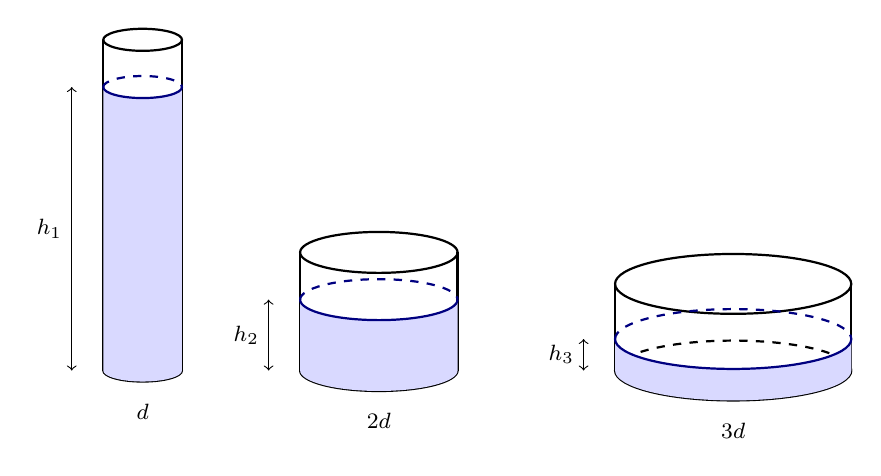
\begin{tikzpicture}[scale=1]
        % --- cilindro 1: semilarghezza 0.5, altezza 4.2, livello 3.6, ry 0.14 ---
        \begin{scope}
            \draw[thick,dashed] (-0.5,0) arc (180:0:0.5 and 0.14);
            \draw[thick] (-0.5,0) arc (180:360:0.5 and 0.14);
            \draw[thick] (-0.5,0) -- (-0.5,4.2)  (0.5,0) -- (0.5,4.2);
            \draw[thick] (0,4.2) ellipse (0.5 and 0.14);
            \fill[blue!15] (-0.5,0) -- (-0.5,3.6) arc (180:360:0.5 and 0.14) -- (0.5,0) arc (360:180:0.5 and 0.14);
            \draw[blue!50!black,thick] (-0.5,3.6) arc (180:360:0.5 and 0.14);
            \draw[blue!50!black,thick,dashed] (-0.5,3.6) arc (180:0:0.5 and 0.14);
            \draw[<->] (-0.9,0) -- (-0.9,3.6) node[midway,left]{\footnotesize $h_1$};
            \node[below] at (0,-0.3) {\footnotesize $d$};
        \end{scope}
        % --- cilindro 2: semilarghezza 1.0, altezza 1.5, livello 0.9, ry 0.26 ---
        \begin{scope}[xshift=3cm]
            \draw[thick,dashed] (-1,0) arc (180:0:1 and 0.26);
            \draw[thick] (-1,0) arc (180:360:1 and 0.26);
            \draw[thick] (-1,0) -- (-1,1.5)  (1,0) -- (1,1.5);
            \draw[thick] (0,1.5) ellipse (1 and 0.26);
            \fill[blue!15] (-1,0) -- (-1,0.9) arc (180:360:1 and 0.26) -- (1,0) arc (360:180:1 and 0.26);
            \draw[blue!50!black,thick] (-1,0.9) arc (180:360:1 and 0.26);
            \draw[blue!50!black,thick,dashed] (-1,0.9) arc (180:0:1 and 0.26);
            \draw[<->] (-1.4,0) -- (-1.4,0.9) node[midway,left]{\footnotesize $h_2$};
            \node[below] at (0,-0.42) {\footnotesize $2d$};
        \end{scope}
        % --- cilindro 3: semilarghezza 1.5, altezza 1.1, livello 0.4, ry 0.38 ---
        \begin{scope}[xshift=7.5cm]
            \draw[thick,dashed] (-1.5,0) arc (180:0:1.5 and 0.38);
            \draw[thick] (-1.5,0) arc (180:360:1.5 and 0.38);
            \draw[thick] (-1.5,0) -- (-1.5,1.1)  (1.5,0) -- (1.5,1.1);
            \draw[thick] (0,1.1) ellipse (1.5 and 0.38);
            \fill[blue!15] (-1.5,0) -- (-1.5,0.4) arc (180:360:1.5 and 0.38) -- (1.5,0) arc (360:180:1.5 and 0.38);
            \draw[blue!50!black,thick] (-1.5,0.4) arc (180:360:1.5 and 0.38);
            \draw[blue!50!black,thick,dashed] (-1.5,0.4) arc (180:0:1.5 and 0.38);
            \draw[<->] (-1.9,0) -- (-1.9,0.4) node[midway,left]{\footnotesize $h_3$};
            \node[below] at (0,-0.55) {\footnotesize $3d$};
        \end{scope}
    \end{tikzpicture}
    \caption{Lo \emph{stesso} volume di liquido versato in cilindri di diametro crescente: l'altezza raggiunta cala con il quadrato del diametro. Con diametro doppio ($2d$) l'altezza è un quarto; con diametro triplo ($3d$), un nono.}
    \label{fig:tre-cilindri}
\end{figure}

\subsection{Un accenno alla fisica}
Molte grandezze fisiche importanti seguono una legge dell'inverso del quadrato: la forza di gravità fra due corpi e l'intensità della luce (o del suono) che arriva da una sorgente diminuiscono con il quadrato della distanza. Raddoppiando la distanza da una lampadina, la luce che ricevi si riduce a un quarto.

\begin{esercizio}
Si versa \SI{1,0}{\litre} di acqua in un cilindro di diametro \SI{8}{\centi\metre}: il livello arriva a circa \SI{19,9}{\centi\metre}. A quale altezza arriverebbe lo stesso litro in un cilindro di diametro \SI{4}{\centi\metre}?\\
\risp{$h \approx \SI{79,6}{\centi\metre}$ (quattro volte tanto)}
\end{esercizio}

\begin{esercizio}
Un sensore misura un'intensità luminosa di \SI{200}{} unità a \SI{1,0}{\metre} da una lampada. Quanto misurerà a \SI{2,0}{\metre}? E a \SI{5,0}{\metre}?\\
\risp{$\SI{50}{}$ unità; \; $\SI{8}{}$ unità}
\end{esercizio}

\section[Riconoscere la relazione]{Riconoscere la relazione da una tabella o da un grafico}\label{sec:riconoscere}

Di fronte a una tabella di dati sperimentali (due colonne, $x$ e $y$), per capire che tipo di relazione lega le due grandezze si procede per tentativi, calcolando una colonna in più:
\begin{elenco}
    \item se resta costante il \textbf{rapporto} $y/x$ \; $\to$ \; proporzionalità \textbf{diretta};
    \item se resta costante il \textbf{prodotto} $x\,y$ \; $\to$ \; proporzionalità \textbf{inversa};
    \item se resta costante il rapporto $y/x^2$ \; $\to$ \; proporzionalità \textbf{quadratica};
    \item se resta costante $y\,x^2$ \; $\to$ \; inversamente proporzionale al quadrato.
\end{elenco}
``Costante'', su dati sperimentali, significa costante \emph{entro gli errori di misura}: piccole oscillazioni sono normali.

Anche il grafico dà un'indicazione immediata, purché si ricordi che è solo un \emph{indizio}:
\begin{center}
\begin{tabular}{ll}
\toprule
andamento del grafico & possibile relazione \\
\midrule
retta per l'origine & diretta \\
curva che scende avvicinandosi agli assi & inversa \\
curva che sale sempre più ripida (dall'origine) & quadratica \\
\bottomrule
\end{tabular}
\end{center}

\begin{figure}[!htbp]
    \centering
    \begin{tikzpicture}
    \begin{axis}[
        width=0.7\linewidth, height=5.2cm,
        xlabel={$x$}, ylabel={$y$},
        xmin=0, xmax=5.3, ymin=0, ymax=13,
        xtick=\empty, ytick=\empty,
        axis lines=left, legend pos=north west, legend cell align=left,
    ]
    \addplot[ocre, very thick, domain=0:5] {2*x}; \addlegendentry{diretta}
    \addplot[blue!60!black, very thick, samples=80, domain=0.75:5] {8/x}; \addlegendentry{inversa}
    \addplot[red!70!black, very thick, densely dashed, samples=60, domain=0:3.3] {x^2}; \addlegendentry{quadratica}
    \end{axis}
    \end{tikzpicture}
    \caption{I tre andamenti a confronto: retta per l'origine (diretta), iperbole discendente (inversa), parabola crescente (quadratica).}
    \label{fig:tre-andamenti}
\end{figure}

\begin{testexample}[\thetcbcounter \, Che relazione è?]
In un esperimento si ottiene la tabella seguente. Che relazione lega $x$ e $y$?
\begin{center}
\begin{tabular}{c|ccccc}
\toprule
$x$ & 1 & 2 & 3 & 4 & 5 \\
$y$ & 12 & 6 & 4 & 3 & 2{,}4 \\
\bottomrule
\end{tabular}
\end{center}
Il rapporto $y/x$ non è costante ($12$; $3$; $1{,}3$; \dots): non è diretta. Proviamo il prodotto:
\[ x\,y: \quad 1\cdot 12 = 12, \quad 2\cdot 6 = 12, \quad 3\cdot 4 = 12, \quad 4\cdot 3 = 12, \quad 5\cdot 2{,}4 = 12. \]
Il prodotto è sempre \SI{12}{}: $x$ e $y$ sono \textbf{inversamente proporzionali}, con $y = 12/x$.
\end{testexample}

\begin{esercizio}
Stabilisci il tipo di relazione: \; $x = 2,4,6,8$ \; e \; $y = 3,6,9,12$.\\
\risp{diretta, $y = 1{,}5\,x$}
\end{esercizio}

\begin{esercizio}
Stabilisci il tipo di relazione: \; $x = 1,2,3,4$ \; e \; $y = 2,8,18,32$.\\
\risp{quadratica, $y = 2\,x^2$}
\end{esercizio}

\begin{esercizio}
Stabilisci il tipo di relazione: \; $x = 1,2,4,5$ \; e \; $y = 40,20,10,8$.\\
\risp{inversa, $x\,y = 40$}
\end{esercizio}

\section{Problemi di riepilogo}

\begin{esercizio}
Il lato di un triangolo equilatero è \SI{6}{\centi\metre} e il suo perimetro \SI{18}{\centi\metre}. Scrivi la relazione fra lato e perimetro e indica la costante di proporzionalità.\\
\risp{$P = 3\,l$, \; $k = 3$}
\end{esercizio}

\begin{esercizio}
Un rubinetto riempie una vasca in \SI{40}{\minute}. Quanto tempo impiegherebbero due rubinetti uguali aperti insieme? E quattro?\\
\risp{\SI{20}{\minute}; \; \SI{10}{\minute}}
\end{esercizio}

\begin{esercizio}
La massa di un foglio di carta è proporzionale alla sua area. Un foglio A4 ($\SI{21}{}\times\SI{29,7}{\centi\metre}$) pesa \SI{5,0}{\gram}. Quanto pesa un foglio A3, che ha area doppia?\\
\risp{\SI{10}{\gram}}
\end{esercizio}

\begin{esercizio}
Un cilindro graduato di base \SI{25}{\centi\metre\squared} contiene \SI{200}{\centi\metre\cubed} di acqua. Di quanto sale il livello se si aggiungono altri \SI{50}{\centi\metre\cubed}?\\
\risp{di \SI{2}{\centi\metre} (da \SI{8}{} a \SI{10}{\centi\metre})}
\end{esercizio}

\begin{esercizio}
Per andare da casa a scuola in bicicletta, Marco impiega \SI{18}{\minute} a \SI{15}{\kilo\metre\per\hour}. Che velocità media dovrebbe tenere per impiegare \SI{12}{\minute}?\\
\risp{\SI{22,5}{\kilo\metre\per\hour}}
\end{esercizio}

\begin{esercizio}
Il volume di un cubo è proporzionale al cubo dello spigolo: $V = l^3$. Se lo spigolo raddoppia, di quante volte aumenta il volume?\\
\risp{$8$ volte}
\end{esercizio}

\begin{esercizio}
Una fotografia $\SI{10}{}\times\SI{15}{\centi\metre}$ viene ingrandita fino a $\SI{30}{}\times\SI{45}{\centi\metre}$. Di quante volte aumenta l'area? E il perimetro?\\
\risp{area $\times 9$; \; perimetro $\times 3$}
\end{esercizio}

\begin{esercizio}
Un gas occupa \SI{5,0}{\litre} a \SI{1,0}{\bar}. A temperatura costante viene portato a \SI{4,0}{\bar}. Qual è il nuovo volume?\\
\risp{\SI{1,25}{\litre}}
\end{esercizio}

\begin{esercizio}
Si versano \SI{0,90}{\litre} di succo in bottiglie cilindriche di diametro \SI{6}{\centi\metre}: il livello arriva a circa \SI{31,8}{\centi\metre}. A quale altezza arriverebbe lo stesso succo in una caraffa cilindrica di diametro \SI{18}{\centi\metre}?\\
\risp{$h \approx \SI{3,5}{\centi\metre}$ (nove volte più bassa)}
\end{esercizio}

\begin{esercizio}
Riconosci il tipo di relazione e scrivi la formula: \; $x = 1,2,3,4,5$ \; e \; $y = 100,25,11{,}1,6{,}25,4$.\\
\risp{inversamente proporzionale al quadrato, $y = 100/x^2$}
\end{esercizio}

\begin{esercizio}
Una candela vista a \SI{2}{\metre} di distanza ha una certa luminosità apparente. A che distanza va portata perché appaia $\tfrac{1}{9}$ altrettanto luminosa?\\
\risp{a \SI{6}{\metre}}
\end{esercizio}

\begin{esercizio}
La corda di una chitarra emette una nota tanto più acuta quanto più è corta: la frequenza è inversamente proporzionale alla lunghezza. Una corda lunga \SI{65}{\centi\metre} dà una nota a \SI{330}{\hertz}. Dove va premuta (quale lunghezza) per ottenere \SI{440}{\hertz}?\\
\risp{$L \approx \SI{48,75}{\centi\metre}$}
\end{esercizio}

\begin{esercizio}
In una tabella $x = 2,3,5,8$ corrisponde a $y = 8,18,50,128$. Che relazione c'è? Quanto vale $y$ per $x = 10$?\\
\risp{quadratica, $y = 2\,x^2$; \; $y = 200$}
\end{esercizio}
